%%%%%%%%%%%%%%%%%%%%%%%%%%%%%%%%%%%%%%%%%%%%%%%%%%%%%%%%%%%%%%%%%%%%%%%%%%%%%%%%
%2345678901234567890123456789012345678901234567890123456789012345678901234567890
%        1         2         3         4         5         6         7         8
%
% Slightly modified by X. Baró for FG2020
%

%\documentclass[letterpaper, 10 pt, conference]{ieeeconf}  % Comment this line out
                                                          % if you need a4paper
\documentclass[a4paper, 10pt, conference]{ieeeconf}      % Use this line for a4
                                                          % paper
\usepackage{FG2020}

%\FGfinalcopy % *** Uncomment this line for the final submission

\IEEEoverridecommandlockouts                              % This command is only
                                                          % needed if you want to
                                                          % use the \thanks command
\overrideIEEEmargins
% See the \addtolength command later in the file to balance the column lengths
% on the last page of the document

% The following packages can be found on http:\\www.ctan.org
%\usepackage{graphics} % for pdf, bitmapped graphics files
\usepackage{booktabs}
\usepackage{graphicx}
\graphicspath{{figures/}}
\usepackage{hyperref}
\usepackage{cite}
%\usepackage{epsfig} % for postscript graphics files
%\usepackage{mathptmx} % assumes new font selection scheme installed
%\usepackage{times} % assumes new font selection scheme installed
\usepackage{amsmath} % assumes amsmath package installed
%\usepackage{amssymb} % assumes amsmath package installed

\def\FGPaperID{****} % *** Enter the FG2020 Paper ID here

\title{\LARGE \bf
Multi-Label Speech Emotion Recognition Using 2D Convolutional Neural Networks
}

%use this in case of a single affiliation
\author{\parbox{16cm}{\centering
    {\large Brian Pho, Thomas Truong, and Svetlana Yanushkevich}\\
    {\normalsize
    Biometric Technologies Laboratory, Department of Electrical and Computer Engineering, University of Calgary, Alberta, Canada\\}}
}

%use this in case of several affiliations
%\author{\parbox{16cm}{\centering
%    {\large Huibert Kwakernaak$^1$ and Pradeep Misra$^2$}\\
%    {\normalsize
%    $^1$ Faculty of Electrical Engineering, Mathematics and Computer Science, University of Twente, Enschede, The Netherlands\\
%    $^2$ Department of Electrical Engineering, Wright State University, Dayton, USA}}
%    \thanks{This work was not supported by any organization}% <-this % stops a space
%}

\begin{document}

\ifFGfinal
\thispagestyle{empty}
\pagestyle{empty}
\else
\author{Anonymous FG2020 submission\\ Paper ID \FGPaperID \\}
\pagestyle{plain}
\fi
\maketitle


%%%%%%%%%%%%%%%%%%%%%%%%%%%%%%%%%%%%%%%%%%%%%%%%%%%%%%%%%%%%%%%%%%%%%%%%%%%%%%%%
\begin{abstract}

A problem with current speech emotion recognition systems is that they can only recognize one emotion, from a set of emotions, in speech. This is a problem because it does not match how people recognize emotions in speech. When people hear speech, they can perceive multiple emotions instead of a single emotion. We address this problem by building a 2D convolutional neural network that can also recognize multiple emotions and it achieves an accuracy of 57.64\%. This model demonstrates a more realistic approach to speech emotion recognition by more closely matching human data.
%\footnote{Code for this paper is available on Github at: \url{https://github.com/Brian-Pho/RVST598_Speech-Emotion-Recognition}}

\end{abstract}


%%%%%%%%%%%%%%%%%%%%%%%%%%%%%%%%%%%%%%%%%%%%%%%%%%%%%%%%%%%%%%%%%%%%%%%%%%%%%%%%
\section{INTRODUCTION}

The field of affective computing studies the development of systems that can recognize, interpret, process, and simulate human affects. A subfield of affective computing, the one that we are interested in, is speech emotion recognition (SER). SER is the problem of recognizing which emotions are present in speech and it is important because of its applications to: call center conversations that improve service quality, speech translation systems that are more accurate at conveying emotions, and robotic pets that are more compassionate \cite{Koolagudi2012}.

\subsection{Literature Review}

SER has historically been approached in two ways: feature engineering (FE) and machine learning (ML). FE is a method of manually extracting desired parameters from the data for use in recognition. For audio, examples of parameters include pitch, energy, and Mel-Frequency Cepstral Coefficients (MFCC) \cite{Rybka2013}. Nassif et al. \cite{Nassif2019} found that most researchers used the MFCC parameter for deep learning models but also recommended other parameters such as Linear Predictive Coding. 

ML is a method of creating models that automatically extract their own parameters for recognition without being manually programmed. Examples include convolutional neural networks (CNN), recurrent neural networks (RNN), and long short-term memory (LSTM). Both approaches are not exclusive and a hybrid approach of FE and ML results in better classification accuracy \cite{Nassif2019}.

A common example of combining both approaches is to convert an audio waveform into a spectrogram using the Short-Time Fourier Transform (STFT) and to feed the spectrogram into a neural network. Papers such as \cite{Engel2019}, \cite{Chen2018}, \cite{Badshah2019}, and \cite{Zhao2019} have demonstrated that this approach is successful for processing audio and for SER.

Current state-of-the-art SER has achieved an accuracy of 52.14\% for the case of speaker-independent, single-label emotions on the IEMOCAP database \cite{Zhao2019}. This result was achieved using a 2D CNN LSTM model where the audio waveform was converted into a log-Mel spectrogram and then fed into the model.

However, this model, and other current models, only consider a single emotion per speech sample and are often only trained on one or two databases. Kim et al. \cite{Kim2018a} is an exception as they consider the multi-label case of SER but they did not use ML and they used visual data on top of audio data. This paper extends upon the current literature by considering the problem of multi-label SER by using four databases to train and test a 2D CNN.

The IEMOCAP \cite{busso_2008} and CREMA-D \cite{cao_2014} databases both include multiple labels for each speech sample but the data is usually discarded by considering the emotion with the majority of votes. We argue that discarding the non-majority votes results in a less realistic SER model, due to not matching human performance and due to the loss of information. For example, in the case of speech translation systems, translating "surprise" speech lacks the nuance of whether the surprise is "surprise-happy" such as the case of receiving a gift, or if it is "surprise-sad" such as the case of receiving news of a tragedy. A single label is not able to capture this nuance compared to multiple labels and this could result in inaccurate or offensive translations.

\subsection{Proposed Approach}

The main idea of this paper is to build a more realistic SER system that can recognize multiple emotions in speech. We approach this problem by using more data and by using a 2D CNN to classify speech samples into multiple emotions. We used four public databases then combined the databases into an a single database by processing all of the speech samples into log-Mel spectrograms. These log-Mel spectrograms were then fed into an eight-layer neural network consisting of four convolutional layers and four dense layers. The final output of the neural network is a list of present emotions.

This paper is outlined as follows:
\begin{itemize}
	\item Section 2 details the methodology we use such as how we combined the four databases and describes the architecture of the neural network.
	\item Section 3 describes and discusses the results from testing the neural network.
	\item Section 4 concludes this paper and provides suggestions for future directions.
\end{itemize}


%%%%%%%%%%%%%%%%%%%%%%%%%%%%%%%%%%%%%%%%%%%%%%%%%%%%%%%%%%%%%%%%%%%%%%%%%%%%%%%%
\section{METHODOLOGY}

We approach the problem of SER by preprocessing samples from four databases and then feeding those samples into a CNN. We preprocess the speech samples into log-Mel spectrogram to help the neural network extract features relevant to emotion recognition. This choice is based on the previous work by \cite{Engel2019} and \cite{Badshah2017} where log-Mel spectrograms were successfully used for extracting audio features. 

The choice to use a CNN is based on the previous work of Balakrishnan et al. \cite{Balakrishnan2017} which found that CNN-based models have superior performance compared to RNNs. Another justification for using CNNs is due to treating the log-Mel spectrograms as images and CNNs have been shown to perform well on images \cite{Krizhevsky2012}. Both the preprocessing steps and the CNN were implemented in Python using the Librosa \cite{McFee2015} and Keras \cite{Chollet2015} libraries respectively.

\subsection{Preprocessing} \label{Preprocessing}

%\begin{table*}
%	\centering
%	\caption{Comparison of databases with their labeled emotions.}
%	\label{dbEmoTable}
%	\begin{tabular}{@{}lccccccccccccc@{}}
%		\toprule
%		Databases & \multicolumn{13}{c}{Emotions} \\ 
%		\cmidrule{2-14}
%		& Neutral & Anger & Disgust & Fear & Happy & Sad & Surprise & Calm & Excitement & Frustration & Amused & Sleepy & Bored \\ 
%		\midrule
%		IEMOCAP & x & x & x & x & x & x & x &   & x & x &   &   &   \\
%		CREMA-D & x & x & x & x & x & x &   &   &   &   &   &   &   \\
%		TESS & x & x & x & x & x & x & x &   &   &   &   &   &   \\
%		RAVDESS & x & x & x & x & x & x & x & x &   &   &   &   &   \\
%		MSP-IMPROV & x & x & x & x & x & x & x &   &   &   &   &   &   \\
%		SAVEE & x & x & x & x & x & x & x &   &   &   &   &   &   \\
%		Emo-DB & x & x & x & x & x & x &   &   &   &   &   &   & x \\
%		EmoV-DB & x & x & x &   &   &   &   &   &   &   & x & x &   \\
%		\bottomrule
%	\end{tabular}%
%\end{table*}
%Table \ref{dbEmoTable} compares the set of emotions of each database which makes it easier to identify overlapping emotions.

To build a more realistic SER system, we first collect speech samples with their labeled emotion. We considered eight databases and chose four based on accessibility and based on the number of overlapping emotions. We chose four databases because it becomes more difficult to maintain consistency in the final samples due to database variability. Databases can vary in
\begin{itemize}
	\item The set and number of labeled emotions
	\item The number of labels per sample
	\item The audio quality such as sampling rate and noise
	\item The spoken language
\end{itemize}
Given this variability, we chose the following four databases: IEMOCAP \cite{busso_2008}, TESS \cite{dupuis_2011}, RAVDESS \cite{livingstone_2018}, and CREMA-D \cite{cao_2014}.

To control for the set and number of labeled emotions, we consider the following seven emotions for recognition: neutral, anger, disgust, fear, happy, sad, and surprise. We chose these seven emotions due to them being considered basic emotions by Ekman \cite{Ekman1992} and due to these seven being the most common among all databases. 

To control for the number of labels per sample, we mixed the multi-labeled data from the IEMOCAP and CREMA-D databases with the single-labeled data from the TESS and RAVDESS databases. We chose to mix of single- and multi- labeled data to increase the number of samples that the model can learn from and because the single-labels can be considered as special cases of multi-labeled data. However, we removed samples that were labeled with four or five emotions because we consider these samples to be ambiguous and because outliers can hinder a neural network's ability to learn. Outliers can hinder a neural network's ability to learn by causing large gradient updates that prevent the model from converging \cite{Chollet2017}.

To control for the audio quality, we resampled all samples to 48 kHz, applied noise reduction to samples from the IEMOCAP and CREMA-D databases, and cropped all samples to 4.5 seconds. We used a kaiser filter for resampling and used spectral gating for noise reduction. We only applied noise reduction to the IEMOCAP and CREMA-D databases after listening to the audio. Lastly, we chose databases that are spoken in English to maintain language consistency.

We combined these four databases into a combined database to train, validate, and test the neural network. Each sample from a database went through the same preprocessing steps to maintain consistency across all samples. The detailed steps are described below.
\begin{enumerate}
	\item A sample starts as a raw waveform in the form of time series points specifying the amplitude at a point in time.
	\item The sample is then padded or cropped to the desired length of 4.5s. Shorter samples were zero-padded on the right tail. Longer samples were right-tail cropped and the extra information was discarded.
	\item If the sample came from a database that we considered noisy, then a noise reduction filter was applied to the sample. We consider the IEMOCAP and CREMA-D databases to be noisy.
	\item The sample is then converted into a log-Mel spectrogram using the STFT and Mel scale. The phase information was discarded as it does not appear to hold relevant information \cite{Kozakowski2017}.
	\item The final step is to normalize the spectrograms to have values between negative one and one. This was done by using a min-max scaling function.
\end{enumerate}

For the STFT, we used a window size of 3072 with a 75\% overlap. This choice is based on the work of Zhao et al. \cite{Zhao2019} where they also use 75\% overlap but with a smaller window size (2048) and they achieved excellent results. 

For the Mel scale, we set the minimum frequency to 20 Hz and maximum frequency to 12 kHz with 200 Mel bins. The frequency range was chosen after experimenting with various ranges and selecting the range that resulted in visually clean spectrograms. The number of Mel bins was also chosen after experimentation as too few bins resulted in poor temporal resolution while too many bins resulted in poor frequency resolution.

\begin{equation}
	\label{minmaxscale}
	\begin{aligned}
		X_{std} &= \frac{X - X_{min}}{X_{max} - X_{min}}\\
		X_{scaled} &= X_{std} \cdot (max - min) + min
	\end{aligned}
\end{equation}

The min-max scaling is defined in (\ref{minmaxscale}) where $X_{min}$ is the smallest value in tensor $X$, $X_{max}$ is the largest value in tensor $X$, $min$ is the lower bound set to $-1$, and $max$ is the upper bound set to $1$. We scaled all spectrograms to only have values between $-1$ and $1$ as this reduces the chances of triggering large gradient updates that prevent the model from converging \cite{Chollet2017}.

%\begin{figure}
%	\centering
%	\hspace{6mm}
%	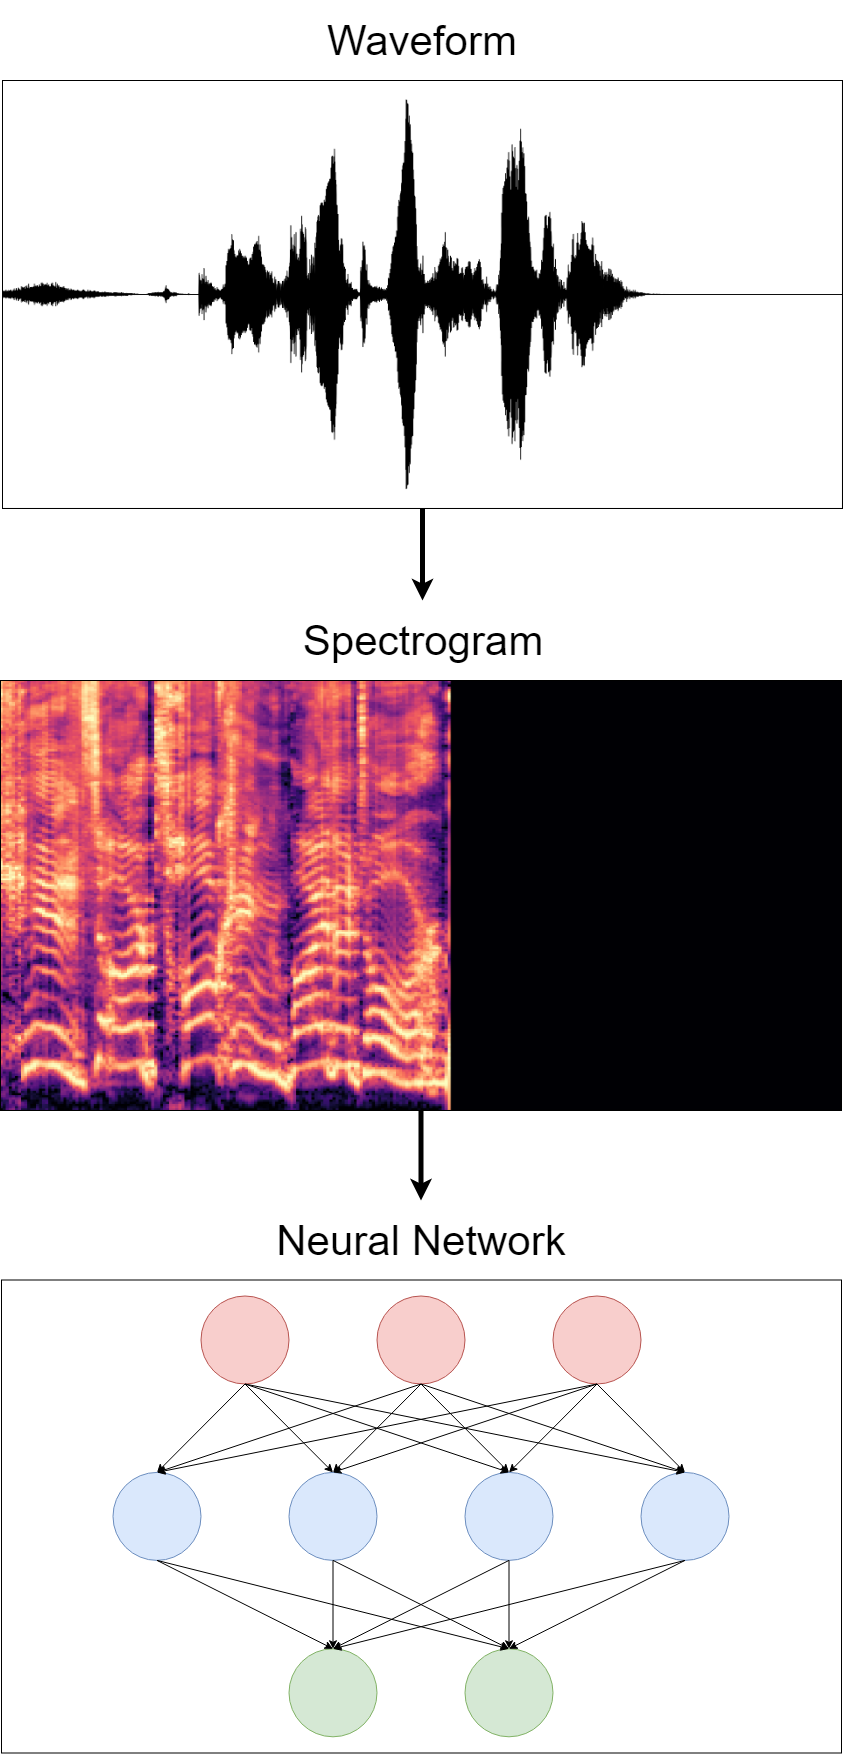
\includegraphics[width=\linewidth]{high_level_dataflow_diagram.png}
%	\caption{High level overview of the processing stages that a speech sample goes through.}
%	\label{highLevelDataFlowDiagram}
%\end{figure}

\subsection{Neural Network}

%\begin{figure*}
%	\centering
%	\hspace{6mm}
%	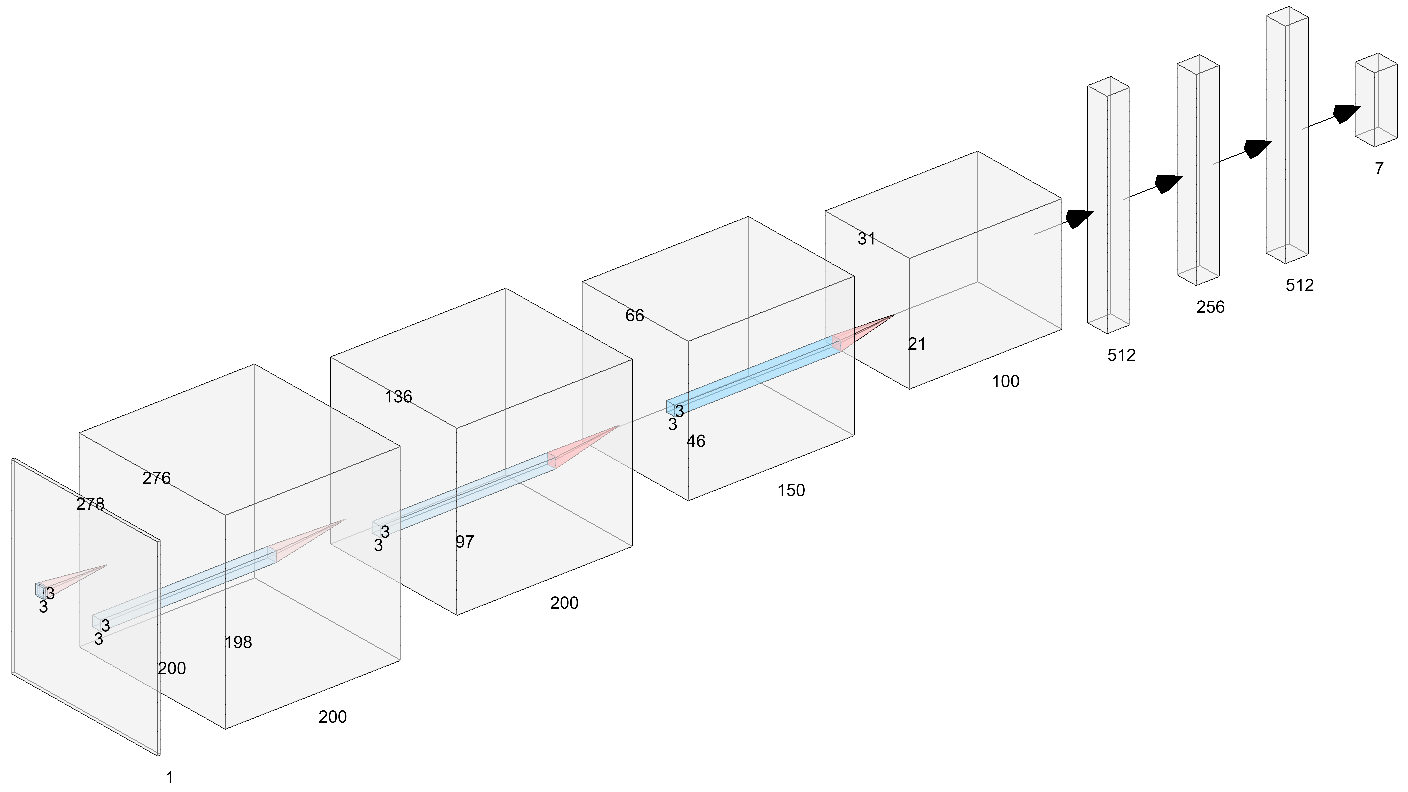
\includegraphics[width=\textwidth]{neural_network_architecture.png}
%	\caption{Architecture for the SER network including the input layer and eight processing layers.}
%	\label{neuralNetworkArchitecture}
%\end{figure*}

\begin{figure}
	\centering
	\hspace{6mm}
	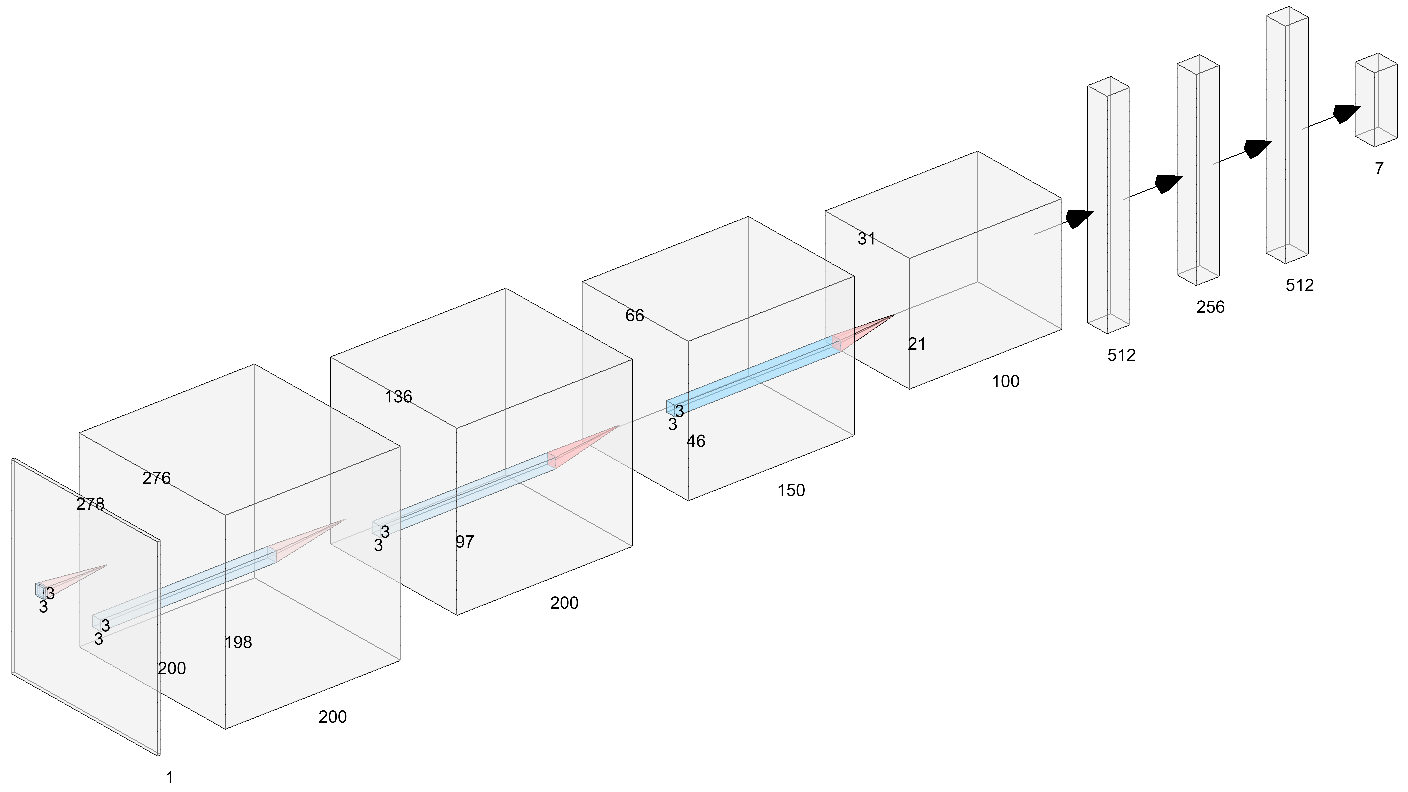
\includegraphics[width=\linewidth]{neural_network_architecture.png}
	\caption{Architecture for the SER network including the input layer and eight processing layers.}
	\label{neuralNetworkArchitecture}
\end{figure}

After all of the databases were processed as described in section \ref{Preprocessing}, the final combined database was fed into a neural network for training, validation, and testing. We constructed an eight layer neural network consisting of four convolutional layers and four dense layers. The network architecture is shown in figure \ref{neuralNetworkArchitecture}. The training process is described below.
\begin{itemize}
	\item We shuffled the combined database to make each input batch more uniform thus mitigating large gradient updates.
	\item We split the combined database into 80\% training, 10\% validation, and 10\% testing.
	\item We applied dropout to the dense layers and batch normalization to the convolutional layers to deal with overfitting \cite{Srivastava2014}, \cite{Ioffe2015}.
	\item We updated the model's hyperparameters based on the validation loss and accuracy to improve the model's accuracy and ability to generalize.
	\item We used class weights during training to address class imbalance.
\end{itemize}

Table \ref{modelHyperparams} describes the model's hyperparameters and table \ref{trainHyperparams} describes the training hyperparameters. The decision to use \textit{binary cross-entropy} as the loss measure is due to multi-label problems considering each output as independent and thus each output acts like a binary classifier. This lets the model only penalize the outputs that are incorrect without penalizing the other outputs. However, we use \textit{categorical cross-entropy} as the accuracy metric because binary cross-entropy would provide the incorrect accuracy as it defined for a binary output such as 0 or 1, not vectors containing binary outputs. Different loss functions should be considered in the future to improve training results.

Likewise, we use \textit{sigmoid} as the output layer's activation function instead of the more commonly used \textit{softmax} function in classification. The justification is the same as in our choice of loss measure; sigmoid treats each output as independent which means multiple outputs can be true while softmax maximizes a single output while minimize all other outputs.

\begin{table}
	\centering
	\caption{The model's hyperparameters.}
	\label{modelHyperparams}
	\begin{tabular}{@{}lr@{}}
		\toprule
		Hyperparameter & Value \\
		\midrule
		Input Dimensions & 278w x 200h x 1d \\
		Optimization Algorithm & Adam \\
		Learning Rate & 0.001 \\
		Beta 1 & 0.9 \\
		Beta 2 & 0.999 \\
		Epsilon & $10^{-8}$ \\
		Loss Measure & Binary Cross-entropy \\
		Accuracy Metric & Categorical Cross-entropy \\
		Hidden Layer Activation Function & ReLU \\
		Output Layer Activation Function & Sigmoid \\
		\bottomrule
	\end{tabular}
\end{table}

\begin{table}
	\centering
	\caption{The training hyperparameters.}
	\label{trainHyperparams}
	\begin{tabular}{@{}lr@{}}
		\toprule
		Hyperparameter & Value \\
		\midrule
		Epochs & 20 \\
		Batch Size & 32 \\
		Training Set & 17,341 \\
		Validation Set & 2,167 \\
		Testing Set & 2,167 \\
		\bottomrule
	\end{tabular}
\end{table}

The final model was evaluated on the testing set by using average accuracy that was calculated from the confusion matrices shown in figure \ref{confusionMatrix}. The confusion matrices are calculated by comparing the true labels to the predicted labels for each independent emotion.

We define accuracy as the unweighted average accuracy of all emotions and this is mathematically described in (\ref{aveacc}) where $n$ is the total number of emotions (7 in our case), $TP_{i}$ is the number of true positives for emotion $i$, $TN_{i}$ is the number of true negatives for emotion $i$, and $Total_{i}$ is the total number of predictions for emotion $i$.

\begin{equation}
	\label{aveacc}
	Accuracy = \frac{\sum_{i=1}^{n}\frac{TP_{i} + TN_{i}}{Total_{i}}}{n}
\end{equation}

In summary, we calculate the accuracy per emotion and then average over these accuracies to obtain the final accuracy. We chose this definition of accuracy so that we can compare our results to other papers that also use a similar measure of accuracy that is calculated from the confusion matrices.

\addtolength{\textheight}{-3cm}   % This command serves to balance the column lengths
                                  % on the last page of the document manually. It shortens
                                  % the textheight of the last page by a suitable amount.
                                  % This command does not take effect until the next page
                                  % so it should come on the page before the last. Make
                                  % sure that you do not shorten the textheight too much.


%%%%%%%%%%%%%%%%%%%%%%%%%%%%%%%%%%%%%%%%%%%%%%%%%%%%%%%%%%%%%%%%%%%%%%%%%%%%%%%%
\section{RESULTS AND DISCUSSION}

After training the model, it was evaluated on the testing set to get the final accuracy. The final accuracy achieved was 57.64\%. Comparisons to the current literature is shown in table \ref{litacccompare}. We compare our results to the single-label case of SER as we could not find papers with results for the multi-label case.

\begin{figure}
	\centering
	\hspace{6mm}
	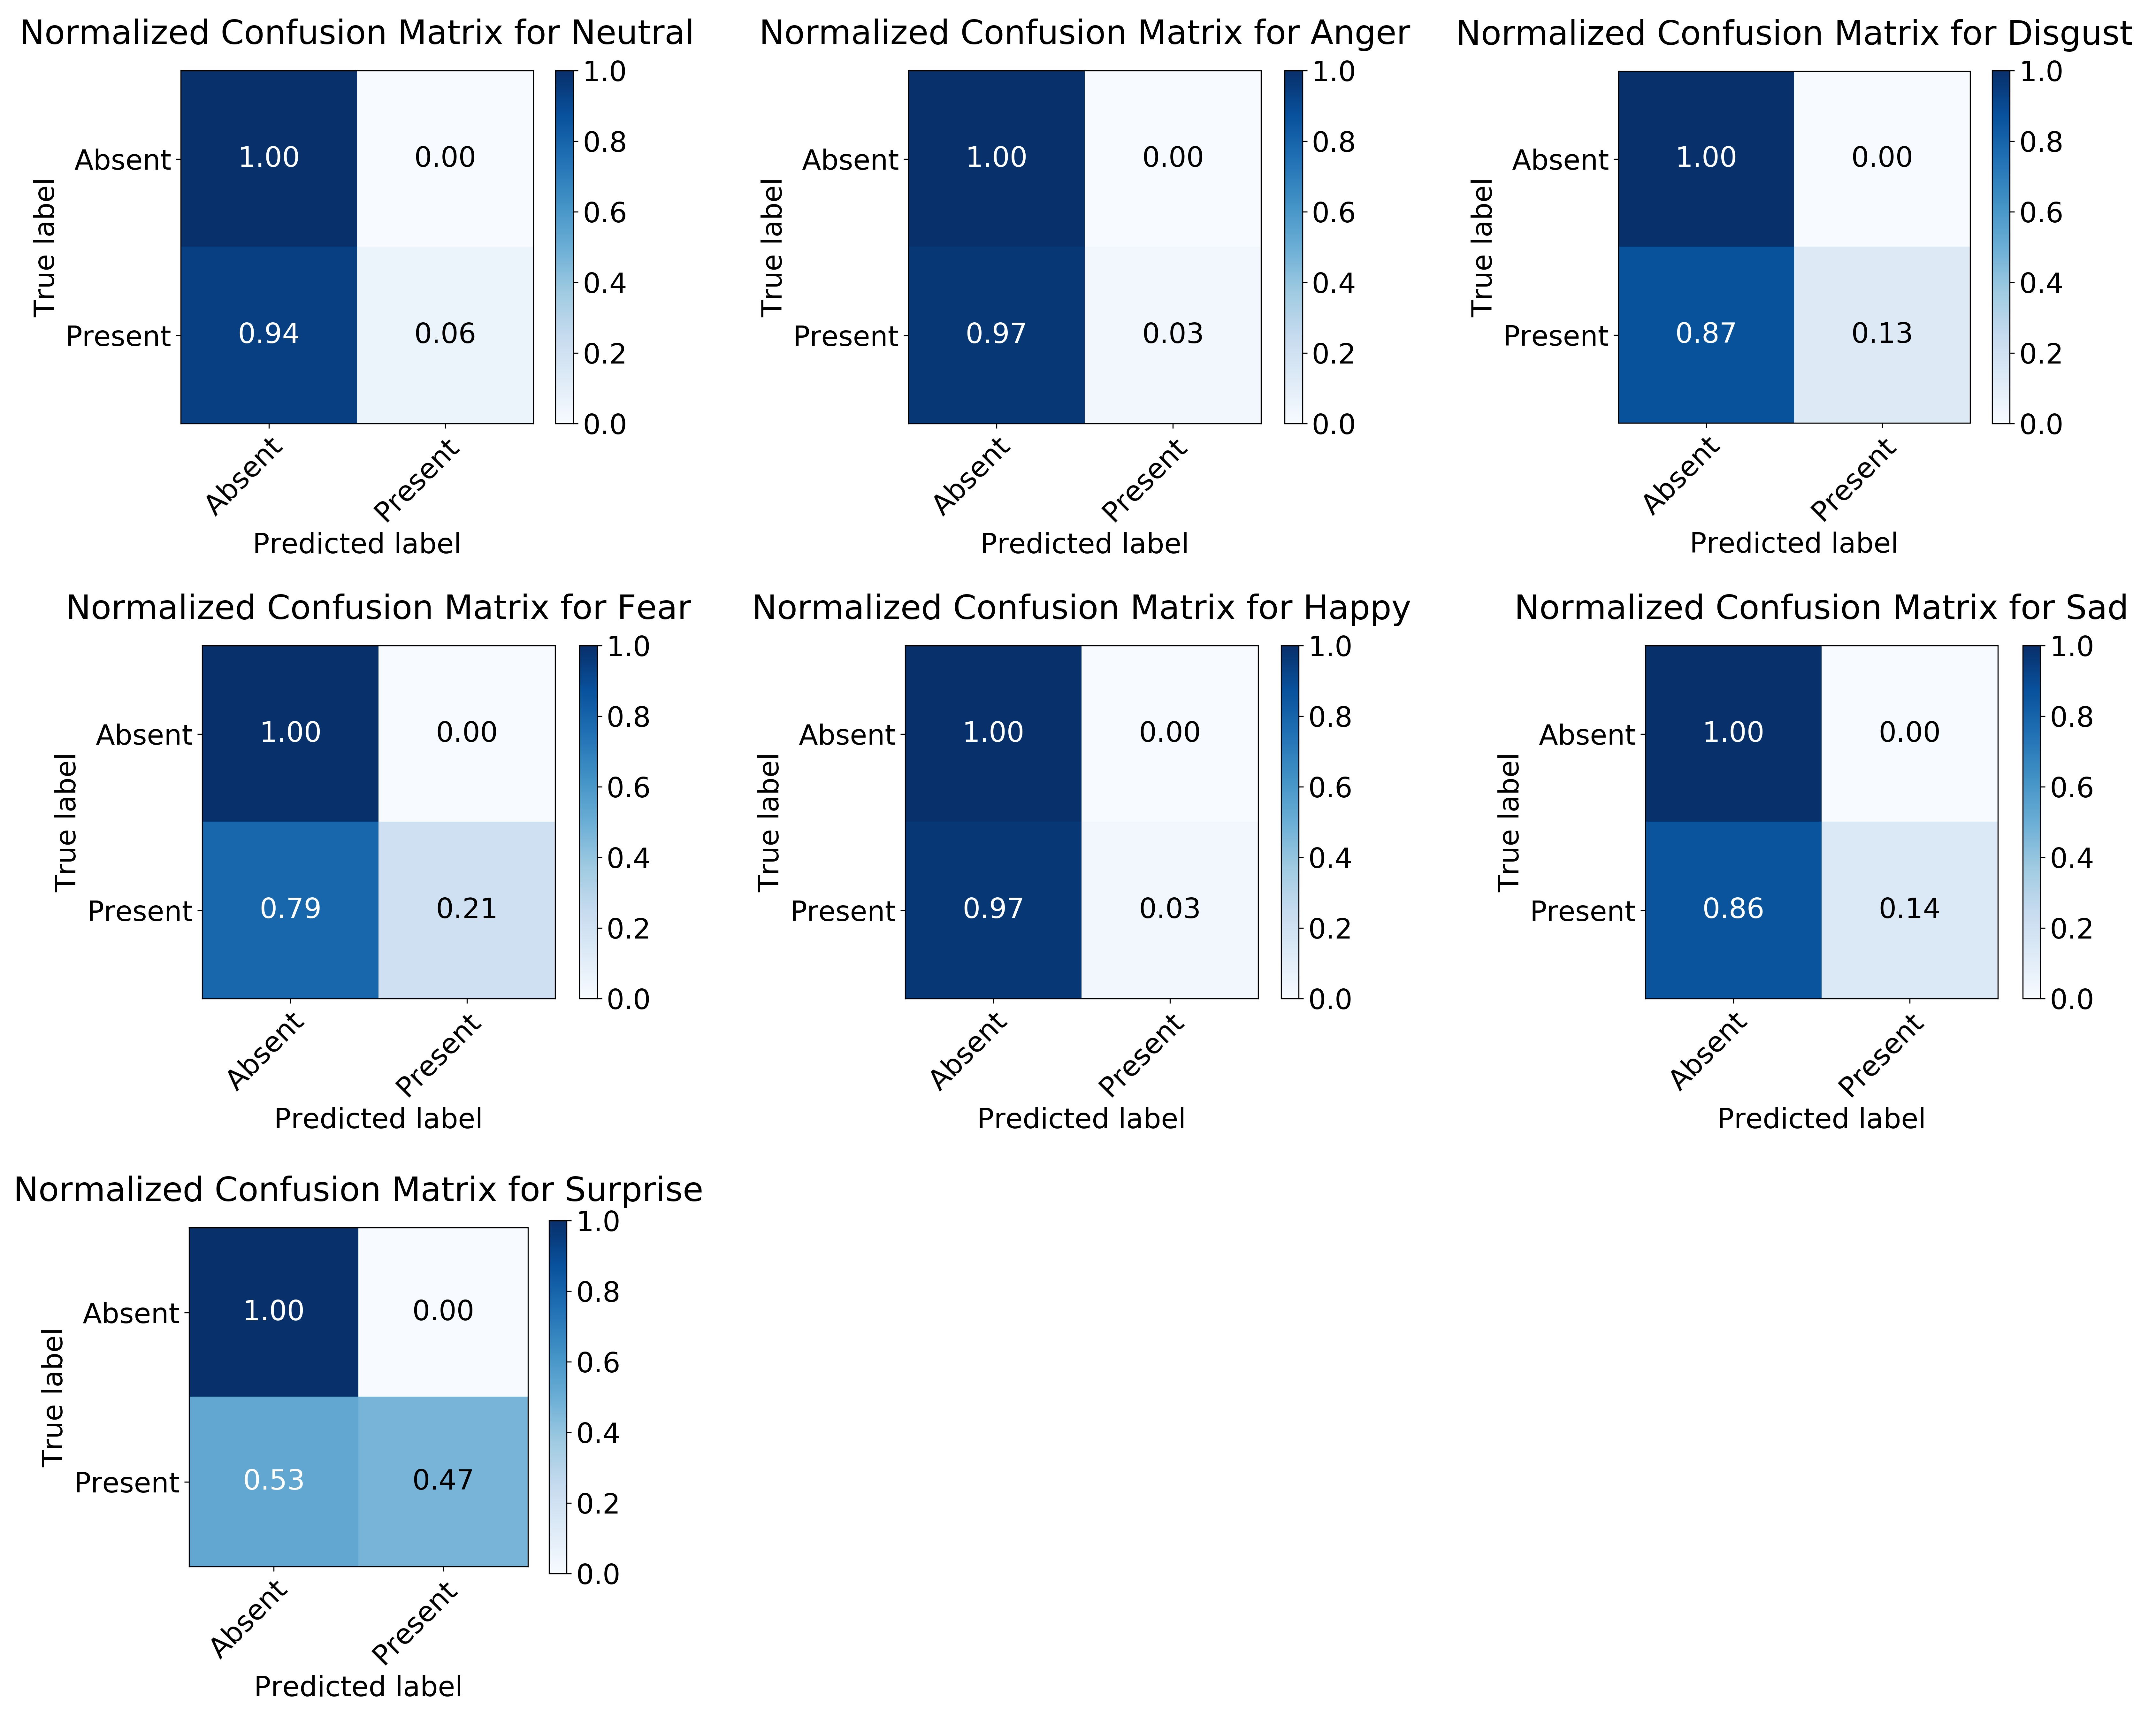
\includegraphics[width=\linewidth]{confusion_matrix.png}
	\caption{Confusion matrices for each emotion.}
	\label{confusionMatrix}
\end{figure}

\begin{table*}
	\centering
	\caption{Comparison of SER accuracy in literature.}
	\label{litacccompare}
	\begin{tabular}{@{}llllllr@{}}
		\toprule
		Research Work & Method & Testing Method & Number of Emotions & Databases Used & Label Type & Accuracy (\%) \\
		\midrule
		Zhao et al. \cite{Zhao2019} & CNN + LSTM & Testing set & 6 & IEMOCAP & Single & 52.1 \\
		Our Work & CNN & Testing set & 7 & \begin{tabular}[c]{@{}l@{}}IEMOCAP, TESS, \\ RAVDESS, CREMA-D\end{tabular} & Multi & 57.6 \\
		Etienne et al. \cite{Etienne2018} & CNN + LSTM & Testing set & 4 & IEMOCAP & Single & 61.7 \\
		Zhang et al. \cite{Zhang2019} & CNN & Testing set & 4 & IEMOCAP & Single & 63.9 \\
		Fayek et al. \cite{Fayek2017} & CNN & Testing set & 4 & IEMOCAP & Single & 64.8 \\
		Yenigalla et al. \cite{Yenigalla2018} & CNN & Testing set & 4 & IEMOCAP & Single & 73.9 \\
		Badshah et al. \cite {Badshah2019} & CNN & Testing set & 7 & Emo-DB, Korean dataset & Single & 80.8 \\
		\bottomrule
	\end{tabular}
\end{table*}

The results achieved in this paper do not reach the state-of-the-art accuracy achieved for the single-label case. But considering how this is the first attempt on the more realistic problem of multi-label SER, we perform reasonably well. Compared to the literature shown in table \ref{litacccompare}, no other paper considers as many emotions as we do while also using four databases and also tackling the multi-label problem. So we conclude that we are successful in building a more realistic SER system by using ML and more data to tackle the problem of recognizing multiple emotions in speech.

In analyzing the confusion matrices, we see that the model predicts an emotion is absent in most of the samples with "surprise" being the exception. We suspect that "surprise" being an exception is due to the class imbalance. The "surprise" class was the least represented class out of the seven classes and this makes the model predict it more due to the use of class weights. Class weights bias the model towards underrepresented classes in an attempt to balance classes but this seems to have affected the model's ability to learn.


%%%%%%%%%%%%%%%%%%%%%%%%%%%%%%%%%%%%%%%%%%%%%%%%%%%%%%%%%%%%%%%%%%%%%%%%%%%%%%%%
\section{CONCLUSION AND FUTURE WORK}

Overall, this paper presented a 2D CNN model that achieved an accuracy of 57.64\% on the problem of multi-label speech emotion recognition using four combined databases. We obtained this result by transforming raw speech samples into log-Mel spectrograms using the STFT and the Mel scale. The log-Mel spectrograms are then fed into an eight layer neural network for classification. While this result is a promising start, we suggest improvements that future work can build upon to improve the accuracy of the model and to expand the scope of emotions considered.

One limitation of this work is that we only considered seven emotions but research has suggested that there are more emotions such as boredom, shame, and triumph \cite{Cordaro2018}. However, one issue with expanding the set of considered emotions is the lack of databases with the labeled emotion.

Another limitation of this work is that all samples are spoken in English so the model is biased towards Anglophones. In theory, the basic emotions are universal across languages and cultures so incorporating databases spoken in different languages, such as the Emo-DB database, would help the model generalize across languages \cite{Burkhardt2005}.

The following list is a suggestion that future work could pursue:
\begin{itemize}
	\item Using more sophisticated neural network architectures such as LSTMs or using more databases.
	\item Incorporating the phase data from the STFT.
	\item Testing a binary relevance approach to this multi-label problem.
	\item Replacing the use of STFT with a wavelet transform.
\end{itemize}
Rana et al. \cite{Rana2016} has also shown that SER systems can be more robust by introducing noise into the samples which is another promising future direction.
 

%%%%%%%%%%%%%%%%%%%%%%%%%%%%%%%%%%%%%%%%%%%%%%%%%%%%%%%%%%%%%%%%%%%%%%%%%%%%%%%%
%\section{ACKNOWLEDGMENTS}
%This work was funded by the PURE award granted by the University of Calgary.


%%%%%%%%%%%%%%%%%%%%%%%%%%%%%%%%%%%%%%%%%%%%%%%%%%%%%%%%%%%%%%%%%%%%%%%%%%%%%%%%
\bibliographystyle{IEEEtran}
\bibliography{IEEEabrv,references}


\end{document}
